\documentclass[tikz,border=15pt]{standalone}

\usepackage{tikz,amsmath,amssymb}

\usetikzlibrary{positioning,fit,shapes,arrows.meta,calc,backgrounds}

% === Academic Color Palette ===
\definecolor{acaBlueLine}{HTML}{6080B0}
\definecolor{acaBlueFill}{HTML}{DBEAFE}
\definecolor{acaGreenLine}{HTML}{30A060}
\definecolor{acaGreenFill}{HTML}{A0D0A0}
\definecolor{acaOrangeLine}{HTML}{D06020}
\definecolor{acaOrangeFill}{HTML}{FFE6CC}
\definecolor{acaPurpleLine}{HTML}{6020D0}
\definecolor{acaPurpleFill}{HTML}{E1D5E7}
\definecolor{acaRedLine}{HTML}{B05050}
\definecolor{acaRedFill}{HTML}{F8CECC}
\definecolor{acaGreyLine}{HTML}{666666}
\definecolor{acaGreyFill}{HTML}{F5F5F5}

\begin{document}

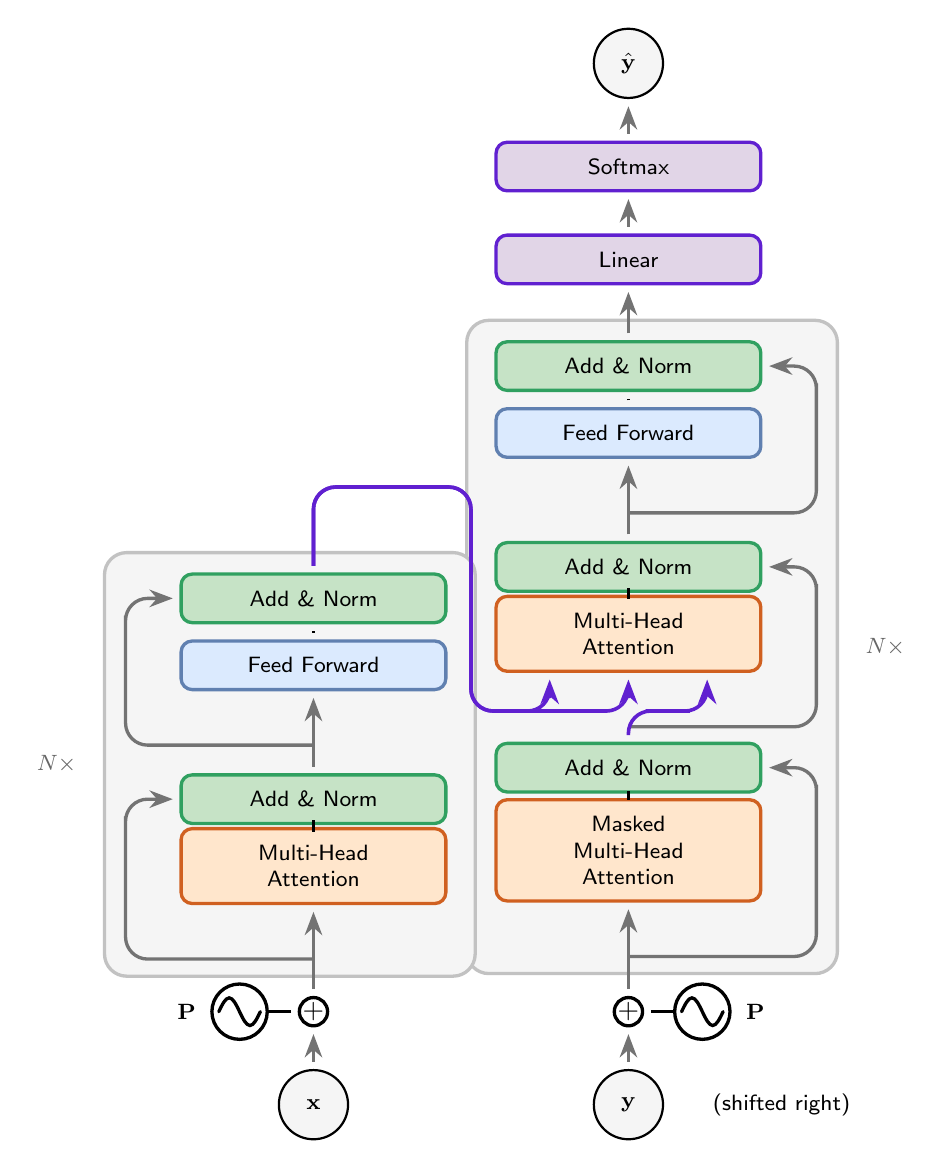
\begin{tikzpicture}[
    >=Stealth,
    very thick,
    arrow/.style={
        ->,
        line width=1.2pt,
        black!55,
        rounded corners=8pt,
    },
    block/.style={
        rectangle,
        fill=acaGreyFill,
        rounded corners=8pt,
        draw=acaGreyLine!40,
        very thick,
    },
    layer/.style={
        rectangle,
        rounded corners=4pt,
        inner xsep=8pt,
        inner ysep=6pt,
        minimum height=1.6em,
        align=center,
        text width=2.8cm,
        draw,
        very thick,
        font=\footnotesize\sffamily,
        outer sep=3pt,
    },
    layer_attn/.style={layer, fill=acaOrangeFill, draw=acaOrangeLine},
    layer_ffn/.style={layer, fill=acaBlueFill, draw=acaBlueLine},
    layer_norm/.style={layer, fill=acaGreenFill!60, draw=acaGreenLine, minimum height=1.2em},
    layer_out/.style={layer, fill=acaPurpleFill, draw=acaPurpleLine},
    input/.style={
        circle,
        minimum width=2.5em,
        draw,
        fill=acaGreyFill,
        thick,
        font=\footnotesize\sffamily,
        outer sep=3pt,
    },
    do path picture/.style={%
        path picture={%
          \pgfpointdiff{\pgfpointanchor{path picture bounding box}{south west}}%
            {\pgfpointanchor{path picture bounding box}{north east}}%
          \pgfgetlastxy\x\y%
          \tikzset{x=\x/2,y=\y/2}%
          #1
        }
    },
    sin wave/.style={do path picture={
        \draw [line cap=round] (-3/4,0)
        sin (-3/8,1/2) cos (0,0) sin (3/8,-1/2) cos (3/4,0);
        }
    }
]

    \node[input] (iemb) at (1.25,-0.45) {$\mathbf{x}$};
    \node[input] (oemb) at (5.25,-0.45) {$\mathbf{y}$};

    % Sum nodes
    \node[circle, draw, minimum size=0.3em, inner sep=0pt, above=1em of iemb, outer sep=3pt] (sum1) {$\mathbf{+}$};
    \node[circle, draw, minimum size=0.3em, inner sep=0pt, above=1em of oemb, outer sep=3pt] (sum2) {$\mathbf{+}$};

    % Positional Encoding
    \node [circle, draw, sin wave, minimum size=2em, left=0.8em of sum1] (pe1) {};
    \node [circle, draw, sin wave, minimum size=2em, right=0.8em of sum2] (pe2) {};

    % === Encoder ===
    \node[layer_attn] (attn1) at (1.25,2.58) {Multi-Head\\Attention};
    \node[layer_norm] (add1) at (1.25,3.43) {Add \& Norm};
    \draw[] (attn1) -- (add1);

    \node[layer_ffn]  (ff1)  at (1.25,5.13) {Feed Forward};
    \node[layer_norm] (add4) at (1.25,5.98) {Add \& Norm};
    \draw[] (ff1) -- (add4);

    % === Decoder ===
    \node[layer_attn] (attn3) at (5.25,2.78) {Masked\\Multi-Head\\Attention};
    \node[layer_norm] (add3) at (5.25,3.83) {Add \& Norm};
    \draw[] (attn3) -- (add3);

    \node[layer_attn] (attn2) at (5.25,5.53) {Multi-Head\\Attention};
    \node[layer_norm] (add2) at (5.25,6.38) {Add \& Norm};
    \draw[] (attn2) -- (add2);

    \node[layer_ffn]  (ff2)  at (5.25,8.08) {Feed Forward};
    \node[layer_norm] (add5) at (5.25,8.93) {Add \& Norm};
    \draw[] (ff2) -- (add5);

    % Nx wrapping boxes
    \coordinate (d1) at ($(attn3.south east) + (0.75,-0.7)$);
    \coordinate (d2) at ($(add5.north west) + (-0.15,0.05)$);
    \coordinate (e1) at ($(attn1.south east) + (0.15,-0.7)$);
    \coordinate (e2) at ($(add4.north west) + (-0.75,0.05)$);
    \begin{scope}[on background layer]
        \node[block, fit=(d1) (d2)] (decoder) {};
        \node[block, fit=(e1) (e2)] (encoder) {};
    \end{scope}

    % Classifier
    \node[layer_out, above=1.5em of add5] (linear) {Linear};
    \node[layer_out, above=1em of linear] (softmax) {Softmax};
    \node[input, above=1em of softmax] (probs) {$\hat{\mathbf{y}}$};

    % Main flow arrows
    \draw[arrow] (add1) -- (ff1);
    \draw[arrow] (add2) -- (ff2);
    \draw[arrow] (add5) -- (linear);
    \draw[arrow] (linear) -- (softmax);
    \draw[arrow] (iemb) -- (sum1);
    \draw[arrow] (sum1) -- (attn1);
    \draw[arrow] (oemb) -- (sum2);
    \draw[arrow] (sum2) -- (attn3);
    \draw[] (sum1) -- (pe1);
    \draw[] (sum2) -- (pe2);
    \draw[arrow] (softmax) -- (probs);

    % Residual connections (curved around components)
    \draw[arrow] (ff1.south)++(0, -0.6) -| ($(add4.west) + (-0.6,-0.5)$) |- (add4.west);
    \draw[arrow] (attn1.south)++(0, -0.6) -| ($(add1.west) + (-0.6,-0.5)$) |- (add1.west);

    \draw[arrow] (attn3.south)++(0, -0.6) -| ($(add3.east) + (0.6,-0.5)$) |- (add3.east);
    \draw[arrow] (attn2.south)++(0, -0.6) -| ($(add2.east) + (0.6,-0.5)$) |- (add2.east);
    \draw[arrow] (ff2.south)++(0, -0.6) -| ($(add5.east) + (0.6,-0.5)$) |- (add5.east);

    % Encoder → Decoder cross-connection
    \draw[arrow,acaPurpleLine,line width=1.3pt] (add4.north) |- ($(add4.north) + (1,1)$) -| ($(add4.north) + (2,-1)$) |- ($(attn2.south) + (-1,-0.4)$) -| ($(attn2.south) + (-1,0)$);
    \draw[arrow,acaPurpleLine,line width=1.3pt] (add4.north) |- ($(add4.north) + (1,1)$) -| ($(add4.north) + (2,-1)$) |- ($(attn2.south) + (0,-0.4)$) -| ($(attn2.south)$);
    \draw[arrow,acaPurpleLine,line width=1.3pt] (add3.north) |- ($(attn2.south) + (0.5,-0.4)$) -| ($(attn2.south) + (1,0)$);

    % Annotations
    \node[font=\footnotesize\sffamily] at ($(oemb.east) + (1.4,0)$) {(shifted right)};
    \node[font=\footnotesize\sffamily] at ($(pe1.west) + (-0.3,0)$) {$\mathbf{P}$};
    \node[font=\footnotesize\sffamily] at ($(pe2.east) + (0.3,0)$) {$\mathbf{P}$};

    % Nx labels
    \node[font=\footnotesize\sffamily\bfseries,acaGreyLine,anchor=east] at ($(encoder.west) + (-0.2,0)$) {$N\times$};
    \node[font=\footnotesize\sffamily\bfseries,acaGreyLine,anchor=west] at ($(decoder.east) + (0.2,0)$) {$N\times$};

\end{tikzpicture}

\end{document}
